\section{Sequence Diagrams}

\subsection{General Sequence}
\begin{figure}[!htb]
    \centering
    \fbox{\includegraphics[width = .98\textwidth, height = .80\textheight]{figures/seq-general.png}}
    \caption{General Sequence}
    \label{fig:seq-general}
\end{figure}

\textbf{explanation}

\subsection{Desktop Client}

\subsubsection{Authentication}
\begin{figure}[hb]
    \centering
    \fbox{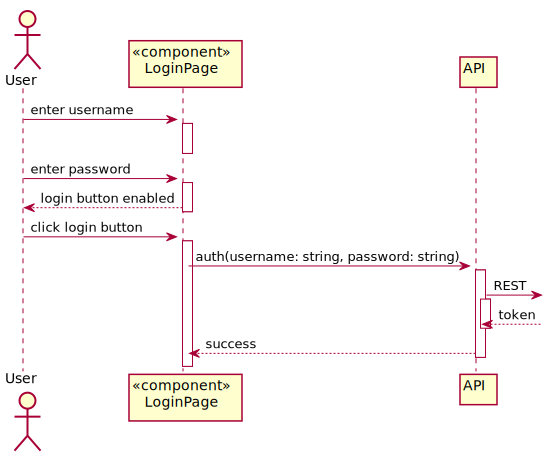
\includegraphics[width = .98\textwidth]{figures/seq-desktop-auth.png}}
    \caption{Authentication Sequence}
    \label{fig:seq-desktop-auth}
\end{figure}

\textbf{explanation}
\newpage

\subsubsection{Workspace Creation}
\begin{figure}[!htb]
    \centering
    \fbox{\includegraphics[width = .98\textwidth]{figures/seq-desktop-workspace-create.png}}
    \caption{Workspace Creation Sequence}
    \label{fig:seq-desktop-workspace-create}
\end{figure}

\textbf{explanation}
\newpage

\subsubsection{Fitting a Sample}
\begin{figure}[!htb]
    \centering
    \fbox{\includegraphics[width = .98\textwidth]{figures/seq-fitting-a-sample.png}}
    \caption{Sample Fitting Sequence}
    \label{fig:seq-fitting-a-sample}
\end{figure}

\textbf{explanation}
\newpage

\subsubsection{Training a Model}
\begin{figure}[!htb]
    \centering
    \fbox{\includegraphics[width = 0.98\textwidth, height = 0.85\textheight]{figures/seq-training-a-model.png}}
    \caption{Model Training Sequence}
    \label{fig:seq-training-a-model}
\end{figure}

\textbf{explanation}


\subsection{Mobile Client}

\subsubsection{Prediction}
\begin{figure}[!htb]
    \centering
    \fbox{\includegraphics[width = 0.98\textwidth, height = 0.80\textheight]{figures/seq-mobile-predict.png}}
    \caption{Mobile Prediction Sequence}
    \label{fig:seq-mobile-predict}
\end{figure}

\textbf{explanation}

\subsection{Authentication}

This diagram shows the registration and validation process of new user accounts. The user first registers with his email, username and a password of his choice and then receives an email that has a validation code. The user enters this token to the desktop client and validates his account.
\subsubsection{Registration and Validation}
\begin{figure}[!htb]
    \centering
    \fbox{\includegraphics[width = 0.98\textwidth, height = 0.78\textheight]{figures/seq-auth-register-and-validate.png}}
    \caption{Registration and Validation}
    \label{fig:seq-auth-register-and-validate}
\end{figure}

\subsubsection{Login}
This diagram shows the login process. The user has already created an account and logs in. The received token is valid for a set amount of time which is then refresh by another token.
\begin{figure}[!htb]
    \centering
    \fbox{\includegraphics[width = 0.98\textwidth, height = 0.78\textheight]{figures/seq-auth-login.png}}
    \caption{Authentication Login}
    \label{fig:seq-auth-login}
\end{figure}

\subsection{Workspace Management}

\subsubsection{Create and Rename Workspace}
In this diagram, the user has no workspace initially. He then access the workspace creation tab of the desktop client. The desktop client asks the server which sensors are available as well as their default and maximum sampling rates. The user chooses the sensors he wishes to use and a name to his workspace. After creating it, the user renames the workspace.
\begin{figure}[!htb]
    \centering
    \fbox{\includegraphics[width = 0.98\textwidth, height = 0.78\textheight]{figures/seq-workspace-create-and-rename.png}}
    \caption{Create and Rename}
    \label{fig:seq-workspace-create-and-rename}
\end{figure}
\newpage

\subsubsection{Submit Sample}
This diagram depicts the sample submission process. To start the sample collection, the desktop client asks for a submission id. After receiving the submission id, it embeds the id to a QR code which is scanned by the mobile client. The mobile client requests the submission config, i.e. which sensors are to be used for the recording and which labels are available. After the recording concludes, the sample is pushed to the server. A new entry for the sample is created in the server database.
\begin{figure}[!htb]
    \centering
    \fbox{\includegraphics[width = 0.98\textwidth, height = 0.78\textheight]{figures/seq-workspace-submit-data.png}}
    \caption{Submit Data}
    \label{fig:seq-workspace-submit-data}
\end{figure}

\subsubsection{Create, Add Description and Delete Labels}
In this diagram, the user creates a new label to use for his samples by choosing a name. He then adds a description to the label. After that, he deletes a label from the workspace which in turn deletes all the samples in the workspace with that label.
\begin{figure}[!htb]
    \centering
    \fbox{\includegraphics[width = 0.98\textwidth, height = 0.78\textheight]{figures/seq-workspace-management.png}}
    \caption{General Workspace Management}
    \label{fig:seq-workspace-management}
\end{figure}

\subsection{Model Management}